% =============================================================================
\section{GHZ states}
% =============================================================================

\copypaste{We also perform mesoscopic Schr\"odinger cat state simulations, corresponding to recent ion-trap experiments with $M$ qubits.
These states violate a genuine multipartite Bell inequality, which means that it is impossible to confine the Bell violation to a microscopic part of the state.
Such inequalities require the measurement of all possible correlation functions at the highest order available.
We find two distinct scaling laws for the total computational difficulty, as measured by the number of samples required to obtain a given sampling error.}


\begin{figure}
    \centerline{%
    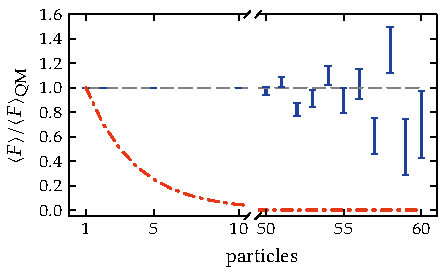
\includegraphics{figures_generated/bell/ghz_violations.pdf}%
    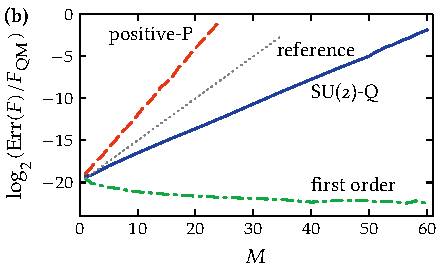
\includegraphics{figures_generated/bell/ghz_errors.pdf}}

    \caption{
    Violations for multi-particle \abbrev{ghz} states.
    (a) Simulated Mermin violation using SU(2)-Q representation.
    The values of expectations and errors are normalized by the quantum mechanical prediction for the corresponding $M$.
    The horizontal grey dashed line gives the quantum prediction.
    The error bars show the sampled result and estimated sampling errors at each value of $M$.
    The red dash-dotted line is the LHV prediction, which gives a Bell violation when above this line.
    Genuine multipartite Bell violations occur for $F_{\mathrm{sample}}/F_{\mathrm{QM}}>1/\sqrt{2}$.
    (b) Relative errors for F (blue line) and first order correlation, or total number of ``spin-ups'' (green dashed line) using SU(2)-Q representation.
    The dotted reference line shows the point at which the sampling errors would give scaling properties as slow as an experimental measurement.}

    \label{fig:bell-ineq:ghz:violation}
\end{figure}


\begin{figure}
    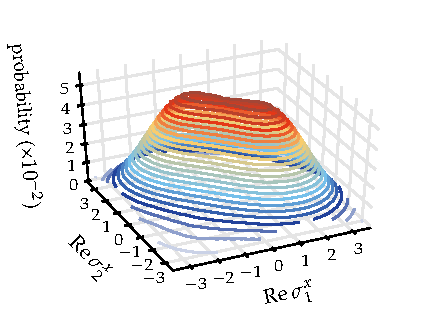
\includegraphics{figures_generated/bell/distribution_P1.pdf}%
    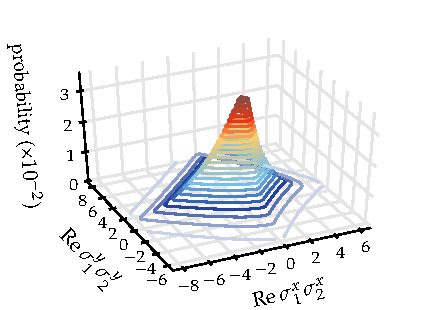
\includegraphics{figures_generated/bell/distribution_P2.pdf}\\
    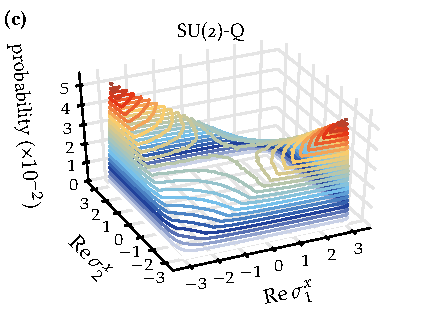
\includegraphics{figures_generated/bell/distribution_Q1.pdf}%
    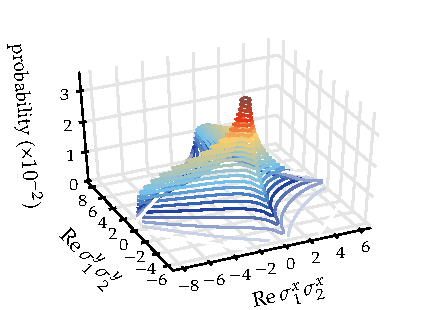
\includegraphics{figures_generated/bell/distribution_Q2.pdf}

    \caption{
    Correlations for the different parts of the quantity $F$, in case of positive-P (a, b) and SU(2)-Q (c, d) representations, $10^{8}$ samples.}

    \label{fig:bell-ineq:ghz:correlations}
\end{figure}

